\authoredSection{julius}{Konzept}
\begin{figure}
	\centering
	\begin{tabular}{@{}c@{\hspace{.5cm}}c@{}}
		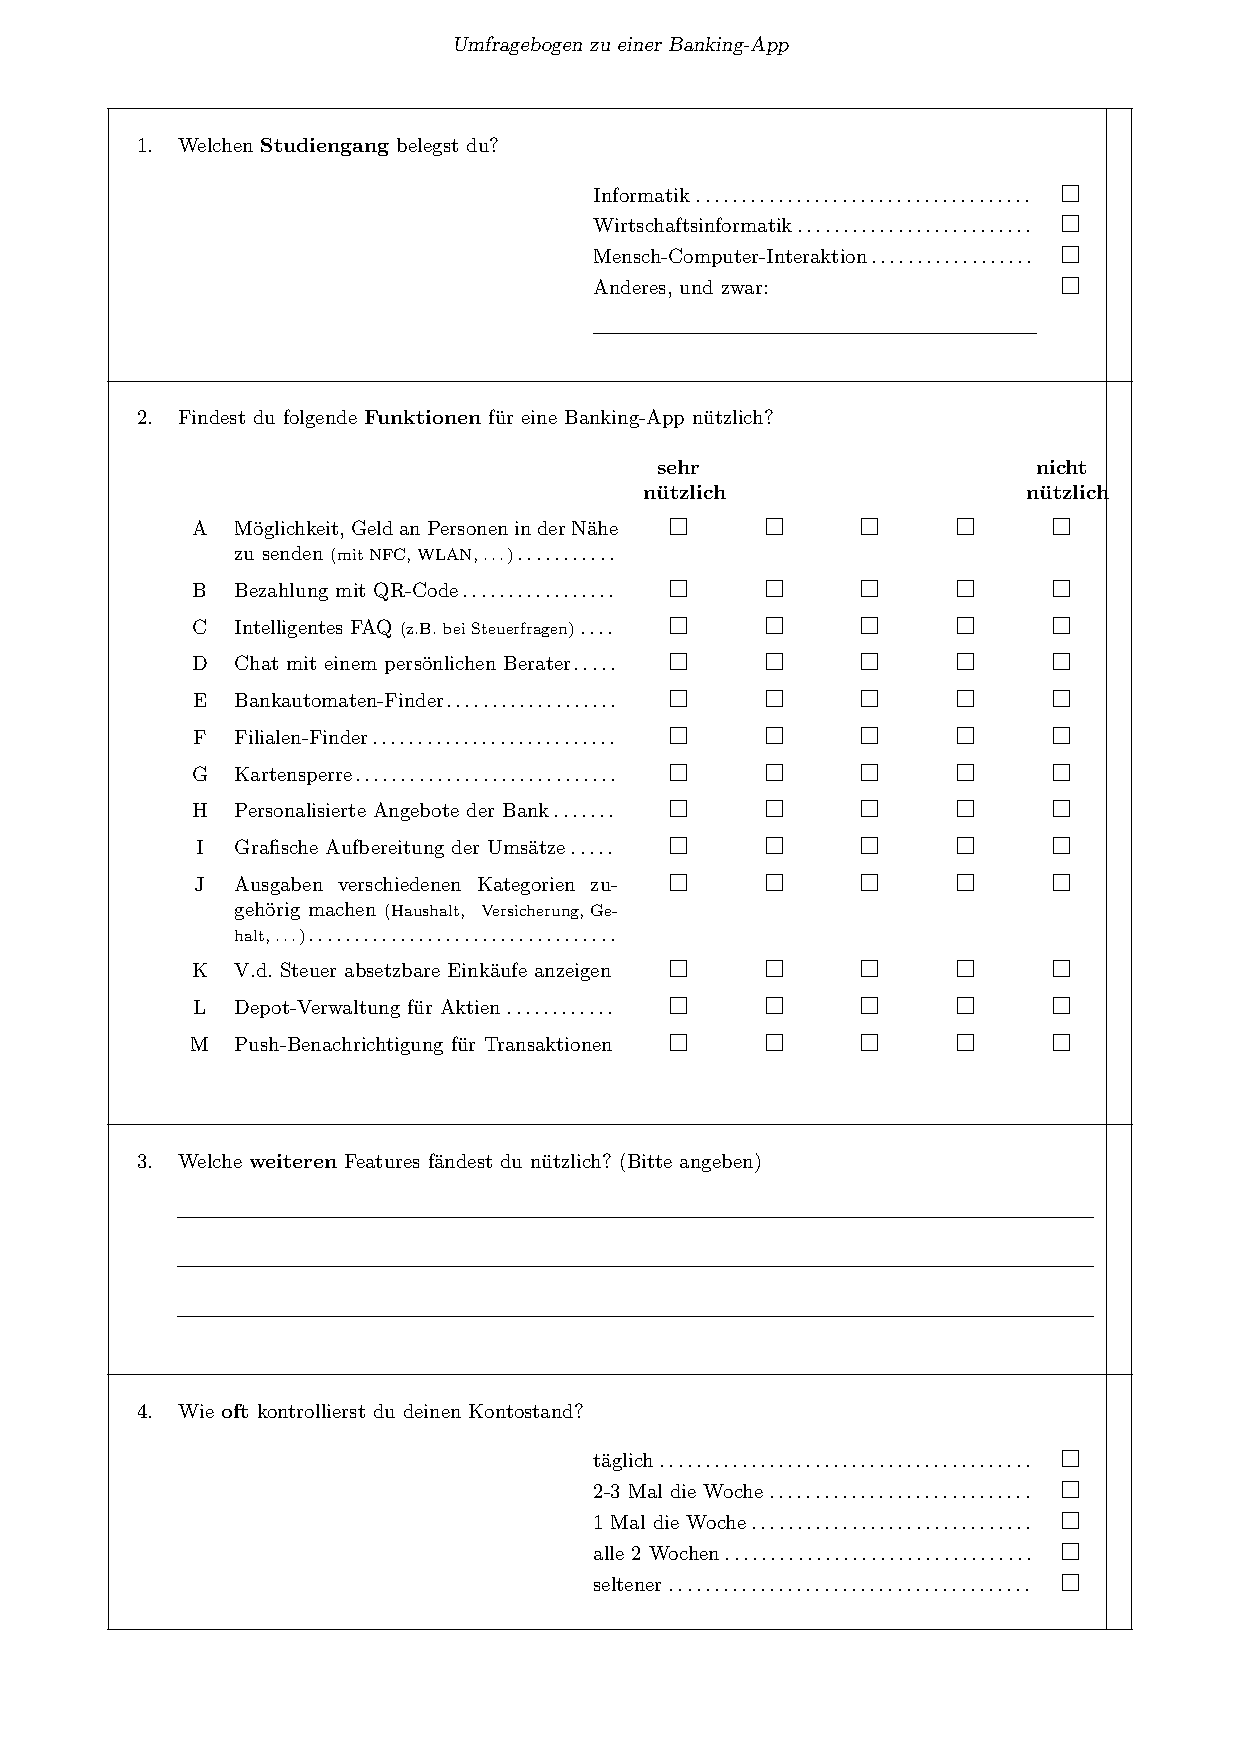
\includegraphics[page=1, height=110mm]{Pictures/Questionnaire} &
		\includegraphics[page=2, height=110mm]{Pictures/Questionnaire}
	\end{tabular}
	\label{fig:Questionnaire}
	\caption{Umfragebogen für erste Ist-Analyse}
\end{figure}
\subsection{Name}
    Der Name der App, "`\textbf{K}i\textbf{B}a"', steht in Anlehnung an eine bekannte Direktbank für eine kundeninteressierte Bank, die mit der Anwendung mehr über ihre Kunden erfahren möchte und mit ihnen in Austausch treten will, um spezifischere Angebote und Beratungen anbieten zu können.
    
\subsection{Gerät}
    Bei der Erstellung eines konkreten Konzepts der Funktionalität haben wir zunächst die Anwendungsfälle besprochen, um die Gerätfrage zu klären. Zweifelsohne gibt es Features, die in einem mobilen Anwendungsfall wahrscheinlicher sind, etwa das Auffinden einer Filiale oder eines Geldautomaten. Eine solche Funktionalität wäre aber nicht filialbankspezifisch. Überhaupt erschien es uns, als wäre der typische Anwendungsfall eher stationär, auf dem Sofa, im Büro, jedenfalls aber in Ruhe. Ein überzeugendes Argument für eine iPad-App ist auch, dass Kunde und Berater in der Filiale zusammen mit der App interagieren und Dinge visualisieren können. Die Vorstellung, ein Kreditangebot auf dem Bildschirm eines iPhones durchzusprechen, ist hingegen eher absurd. 
    
    
    Somit überwogen in der Gruppe ganz eindeutig die Argumente für eine iPad-Anwendung. Zudem war es Aufgabe, eine Vision für die Banking-App der Zukunft zu entwickeln. Der Trend geht unserer Meinung nach zum ubiquitären W-Lan; so gibt es beispielsweise Bestrebungen, öffentliche Netzwerke in der Innenstadt einzurichten. Insofern darf davon ausgegangen werden, dass die mobile Konnektivität zukünftig auch beim iPad zukünftig unproblematisch ist und somit webbasierte Funktionalität auch unterwegs gegeben ist.
    

\subsection{Funktionen}
    Die Kernfunktionen der App sollen sich auf genau die Bereiche konzentrieren, die einer Direktbank nicht zur Verfügung stehen und somit nicht trivial nachgebaut werden können. Dabei haben wir im Zuge der Plenumsdiskussionen und anschließenden internen Debatten insbesondere den zeitlichen Aspekt als zentrale Komponente identifziert. Viele Bescheinigungen und Unterlagen im täglichen Leben werden auch heute noch konkret ausgedruckt benötigt. Der typische Ablauf einer Direktbank sieht so aus, eine Anfrage (etwa nach Wertpapierzweitschriften) per Kontaktformular abzuschicken und dann einige Tage auf die entsprechenden Ausdrucke zu warten. Unsere Idee besteht in einer Self-Service Station innerhalb der Bank, die das Konzept bestehender Automaten erweitert. Ein Kunde kann sein Ipad auf eine Ablage legen und sich mit der Station verbinden. Die Station beinhaltet einen Multifunktionsdrucker und per App können verschiedenste Bescheinigungen ausgedruckt werden. 
    
    Ein wesentliches Produkt von Filialbanken ist das klassische Sparbuch. Umbuchungen können üblicherweise nur in einer Filiale vorgenommen werden, überwiesen werden kann nur auf das Sparkonto. Die Greifbarkeit des Sparbuches vermittelt konservativen, besorgten Sparern ein Gefühl von Sicherheit. Gleichzeitig kann es aber durch diese funktionale Einschränkung auch zu unerwünschten Situationen kommen: ist etwa durch eine Fehlkalkulation an einem Samstagabend kein Geld mehr auf dem Girokonto, muss bis zur Öffnung einer Filiale am Montag gewartet werden, um Guthaben umbuchen zu können. Um dem Vorzubeugen, soll über die Self-Service Station auch Geld umgebucht werden können. Da die Station im Vorraum der Filiale steht, ist sie ganztägig zugänglich. Auf diese Weise bleibt einerseits das Sparbuch als vertrauenswürdige Marke erhalten, die in der Wahrnehmung misstrauischer Benutzer von den Verwerfungen der Online-Kriminalität unberührt bleibt, andererseits ist die Verfügbarkeit erheblich verbessert.
    
    Ebenfalls auf die Bereitstellung von Service-Dienstleistungen zielt der interaktive Filialfinder ab. Aus der Karte heraus sollen Anfragen an eine bestimmte Filiale in der Umgebung er möglicht werden, indem etwa ein Beratungstermin reserviert wird und dann ohne Anstehen erfolgen kann. Eine Funktionalität dieser Art ist 
      
    Als Startbildschirm für die App ist ein Dashboard vorgesehen, das einen graphischen Überblick über Vermögensverlauf und Transaktionen bereitstellt. Hilfreich war hier die Überlegung, dass die meisten Benutzer ihren Kontostand grob kennen und weniger an einer Zahl als vielmehr an den Entwicklungen interessiert sind. Ist der Benutzer nicht eingeloggt, erscheint an dieser Stelle ein Mockup mit der Aufforderung, sich einzuloggen.
    
    Das Kerngeschäft von Filialbanken besteht in der Finanzierung, etwa für Eigenheime. Im Zentrum unserer Überlegungen stand dann auch die Frage, wie eine App dabei helfen kann, diese Dienstleistung für den Endkunden zu verbessern. Im Ergebnis möhten wir einen individualisierten Kreditrechner anbieten, der den App-Benutzer in die Lage versetzt, mittels individuell berechneter Profildaten für sich selbst Finanzierungsrechnungen durchzuführen. Die Idee dahinter ist, dass ein Kunde zunächst für sich selbst einige Finanzierungsvarianten durchspielen kann. Hat er sich eine Variante überlegt, kann ein Termin mit dem persönlichen Berater vereinbart werden und dabei optional gleich der Finanzierungsvorschlag exportiert werden. Im Filialgespräch kann der Berater dann noch individuelle Ratschläge bezüglich Laufzeit und Umfang einer Finanzierung geben.
    
	Eng zusammenhängend mit dem Finanzierungsprofil steht die Aktivierung ("`Authentifikation"') der App in einer Filiale. Ohne eine solche Aktivierung steht dem Benutzer nur passive Funktionalität zur Verfügung, also etwa der Filialfinder und die Umsatzanzeige. Um die App voll nutzen zu können, muss der Benutzer in eine KiBa-Filiale und von einem Berater einen Sicherheitscode eingeben lassen. Ähnlich einer Kreditkarte soll dann bei Gerätverlust auch die App selbst jederzeit gesperrt werden können. Insbesondere dient die Aktivierung aber auch dazu, den Kunden in einem Beratungsgespräch besser kennenzulernen und in einer bankseitigen Datenbank einen persönlichen Ansprechpartner festzuhalten. Aus der App kann dann direkt ein Termin mit dem eingetragenen Berater vereinbart werden. Auch ein Nachrichten-System ist denkbar, um einzelne Fragen direkt zu klären.